\chapter{Esquemas clásicos de control bilateral }




\section{Esquema de Control Posición-Posición}
En esta sección se realiza en primer lugar un análisis teórico de la estabilidad y de la percepción por parte del operador en este esquema de control en sus casos extremos, por ejemplo en el espacio libre donde la impedancia del entorno es nula $(K_e=0)$, el esclavo se mueve libremente, y la única fuerza externa que actúa sobre el sistema es la del operador sobre el mismo maestro. Por el contrario cuando hay una colisión del esclavo con un objeto rígido la impedancia del entorno cambia a $K_e=\infty$\\

Posteriormente se presentarán algunos resultados obtenidos en la plataforma experimental

%\section{Percepci\'on del Entorno por Parte del Operador}
%\section{Influencia del Entorno $E(s)$}
%\section{Influencia de la Din\'amica del Esclavo}
%\section{Influencia de la Din\'amica del Maestro}
%\section{Error en r\'egimen Permanente}
%\section{Esquema de Control Fuerza-Posici\'on}
%\section{An\'alisis del Esquema Fuerza-Posici\'on}
%\section{Percepción del Entorno}
%\section{Influencia del entorno $E(s)$}
%\section{Influencia de la Din\'amica del Esclavo}
%\section{Influencia de la Din\'amica del Maestro}
%\section{Error en Estado Estacionario}
%\section{Implementaci\'on del Esquema Fuerza Posición}
%\section{Conclusiones}
%\chapter{Esquemas de control bilateral con retardo temporal}

%\section{Arquitectura de la Plataforma Experimental de Teleoperaci\'on}
%\section{Implementaci\'on de Algoritmos de Control}
%\section{Arquitecturas Derivadas}
%\section{Arquitectura General del Sistema Teleoperado}




%\chapter{Evaluación de distintas Arquitecturas de Control}

% continuación se muestran los resultados de la evaluación de distintas arquitecturas de control en la plataforma abierta de teleoperación


\section{Control Posición-Posición}

\section{Control Fuerza-Posición}

\section{control híbrido fuerza-fuerza, posición-posición}



\section{RaPA: Rate-Position Architecture}

A continuación se describe una arquitectura de teleoperación híbrida que combina control en velocidad y control de posición para permitir el manejo de un robot esclavo con un espacio de trabajo amplio. Se utiliza información háptica para informar al operador cuando un cambio en el modo de  funcionamiento ha ocurrido . El controlador propuesto permite la realización de  tareas en áreas de trabajo grandes usando un dispositivo háptico con un espacio de trabajo reducido como el PHAMTHOM. Se han realizado experimentos utilizando un robot esclavo virtual simulado con ODE. Una tarea real para la instalación IFMIF ha sido simulada. Dicha tarea tiene por objeto medir los niveles de radiación de materiales en entornos nucleares. Además la arquitectura propuesta se ha comparado con el esquema clásico de control en posición en una tarea de \textit{Pick and Place}, donde se ha comparado la utilidad del método con mejores tiempos en la ejecución de la tarea. Los resultados obtenidos con esta arquitectura han sido publicados por 

\subsection*{Antecedentes}
En la teleoperación , dos modos de control se ha utilizado generalmente para guiar un robot: control de posición y control de velocidad. La decisión de utilizar uno u otro de los modos está principalmente influenciada por las características de la tarea y del los dispositivos maestro y esclavo. Varios trabajos se han llevado a cabo para determinar como la ejecución de la tarea se ve afectada por el modo de control. En [66] los autores han encontrado que el control de posición puede ser 1.5 veces más rápido que el control de velocidad cuando el espacio de trabajo del maestro y del esclavo son similares. Por el contrario, el control de velocidad alcanza mejor un rendimiento cuando el espacio de trabajo del esclavo es mayor que el del maestro.\\
En general, el control de posición ha demostrado ser más adecuado para tareas que involucran movimientos cortos y precisos. Por otra parte, el control en velocidad ha demostrado tener un mejor rendimiento para realizar tareas  que implican movimientos largos y precisos en un gran entorno. Un ejemplo de control en velocidad puede ser la operación manual de una grúa, considerando la grúa como dispositivo esclavo, y las palancas de control como dispositivo maestro, generalmente se usa una palanca para controlar cada grado de libertad, y los movimientos de la misma definen la velocidad y dirección de cada uno de las articulaciones.\\

Por otro lado el control de posición se usa con gran frecuencia en aplicaciones de robótica donde se espera que los movimientos del esclavo imiten los ejecutados por el dispositivo maestro. Como se ha mencionado, este tipo de control es mejor cuando los dispositivos maestro y esclavo tienen espacios de trabajo parecidos, lo cual implica una relación cinemática directa entre dichos dispositivos.\\

En la actualidad, los sistemas comerciales de teleoperación no permiten la combinación del control de posición y el control de velocidad. De hecho cuando hay una diferencia considerable entre los espacios de trabajo de los dispositivos, se utiliza el control de velocidad, o el control de posición con indexación del espacio de trabajo. Indexar el espacio de trabajo del maestro consiste en desvincularlo del esclavo cuando el maestro llega a algún límite mecánico. El dispositivo maestro es trasladado a una nueva posición para permitir que el proceso continúe. Una desventaja de la indexación es que genera desorientación en el operador debido al cambio al cambio en los marcos de referencia, y por tanto la productividad del sistema se ve afectada debido a la inactividad del operador al acostumbrarse a las nuevas referencias.\\

Sin embargo, algunos enfoques que hacen un control híbrido de velocidad-posición se han desarrollado para robots móviles, y aplicaciones hápticas virtuales. En el campo de los robots esclavos con un sistema de referencia fijo (sin plataformas móviles), se referencia al lector a [69] donde se han revisado varios trabajos de este tipo. Además en [69] se ha propuesto un sistema híbrido reconfigurable donde el controlador basado en eventos se utiliza para determinar el cambio en la configuración del sistema. Otros métodos típicos de escalado e indexación requieren que el usuario pulse algún botón para pasar de un modo a otro, sin embargo el algoritmo aquí propuesto no requiere botones para cambiar el modo de control. Debido a estas características, el método propuesto se considera más intuitivo para los operadores, ya que puede fluir de manera más natural de un modo de control a otro.

\subsection*{Descripción del Algoritmo}
El algoritmo propuesto permite cambiar entre el modo de control de posición y el modo de control de velocidad. Dicho cambio se realiza de manera automática sin necesidad de utilizar botones o movimientos especiales. con el fin de mantener al operador informado de las transiciones entre un modo de control en posición y un modo de control en velocidad se utiliza información háptica.

\begin{figure}
\centering
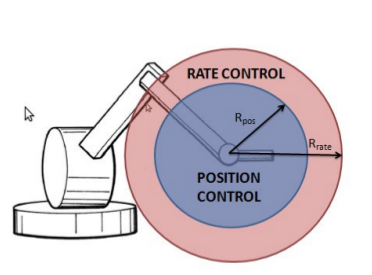
\includegraphics[scale=0.6]{FiguresSoA/Rapa}
\caption{Zonas de control en posición y control en velocidad}
\label{Phamthomrapa}
\end{figure}


El espacio de trabajado del dispositivo háptico maestro ha sido dividido en una zona de control en posición y una zona de control en velocidad como se muestra en la figura. Esto implica que se conseguirá una mayor precisión cunado el robot esclavo es controlado utilizando la zona de posición. Además es posible realizar grandes desplazamientos utilizando la zona de velocidad. Como resultado de  la combinación  de estos dos métodos es posible realizar tareas de precisión en un espacio de trabajo amplio utilizando un dispositivo maestro de tamaño reducido.

\subsection*{Estados del Algoritmo}

Diferentes estados del algoritmo han sido definidos con el fin implementar las transiciones de posición a velocidad y viceversa. En la figura se muestran los estados y como el algoritmo RaPA avanza de un estado al otro dependiendo de los eventos que ocurren durante la teleoperación. algunos de estos han sido configurados para informarle al operador de manera háptica los cambios que han ocurrido en el modo de control y el estado actual del robot remoto (esclavo). Adicionalmente se han definido transiciones entre los estados con el fin de asegurar la estabilidad del sistema.




